\chapter{Fonctions d'une variable réelle}
\labch{fonction_une_variable_reelle}

\textsl{
(texte de \cite{oraux_x_ens_3})\\
À partir du \textsc{xvii}$^\me$ siècle, le développment du calcul infinitésimal, motivé par de nombreux problèmes de cinématique, de mécanique, ou de calcul des variations, fait de la \say{ fonction } l'objet central des mathématiques modernes, alors que jusque là, le \say{ nombre } était la base de l'édifice mathématique. Nous devons à \textsc{Bernoulli} et \textsc{Leibniz} le terme même de \say{ fonction }: pour \textsc{Bernoulli} (1698), une fonction de la variable $x$ est \say{ une quantité formée d'une manière quelconque à partir de $x$ et de constantes }. L'écriture $y = f(x)$ est introduite par \textsc{Euler} en 1734. Les fonctions sont représentées par des courbes dans le plan et \textsc{Euler} se demande si une courbe donnée correspond toujours à une fonction. C'est lui qui distingue les courbes continues, des courbes discontinues, qui sont le plus souvent, à cette époque, des graphes de fonctions continues par morceaux. Cette double conception des fonctions, comme expressions analytiques ou comme graphes du plan, ne sera pas vraiment éclaircie avant le \textsc{xix}$^\me$ siècle (c'est \textsc{Dirichlet} qui donnera la définition moderne d'une fonction comme correspondance; il proposera ainsi (en 1837) un exemple de fonction discontinue partout, la fonction $\chi$ définie par $\chi(x) = 1$ pour $x$ rationnel et $\chi(x)=0$ pour $x$ irrationnel). \textsc{Lagrange}, cherchant à établir les fondements de l'Analyse, s'en tient au point de vue formel et refuse de se référer à toute notion de limite. Ces hésitations empêchent les mathématiciens du \textsc{xvii}$^\me$ siècle  de mener jusqu'à leur achèvement certains de leurs travaux, comme l'étude de l'équation des cordes vibrantes. C'est la génération suivante, avec entre autres \textsc{Gauss}, \textsc{Cauchy}, \textsc{Bolzano} et \textsc{Abel}, qui donnera dans la première moitié du \textsc{xix}$^\me$ siècle un statut rigoureux aux notions de convergence, de continuité, \dots Quant au concept de limite d'une fonction numérique, on doit sans doute sa première définition précise à \textsc{Weierstrass}. 
}


\newpage

\section{Point fixe d'une fonction de \texorpdfstring{$[0, 1] \rightarrow [0, 1]$}{[0, 1] dans [0, 1]}}
\begin{exercice}
    Soit $f$ une fonction dérivable sur $[0, 1]$ telle que:
    $$f(0) = f'(0) = f'(1) = 0 \text{ et } f(1) = 1.$$
    Montrer qu'il existe $c \in ]0, 1[$ tel que $f(c) = c$. 
\end{exercice}

\begin{elem_sol}
    \begin{itemize}
        \item Poser $g(x)= f(x) - x$.
        \item L'objectif est de montrer que $g$ s'annule au moins une fois sur $[0, 1]$ en montrant l'existence de $x_0$ et $x_1$ dans $[0, 1]$ tels que $g(x_0) < 0$ et $g(x_1) > 0$ pour pouvoir appliquer le \textbf{théorème des valeurs intermédiaires}.
        \item Raisonner par l'absurde sur l'existence de $x_0$ et de $x_1$ et écrire la dérivée de $f$ comme la limite de son taux d'accroissement pour aboutir à des contradictions. 
    \end{itemize}
\end{elem_sol}

\begin{marginfigure}[-8cm]
\centering
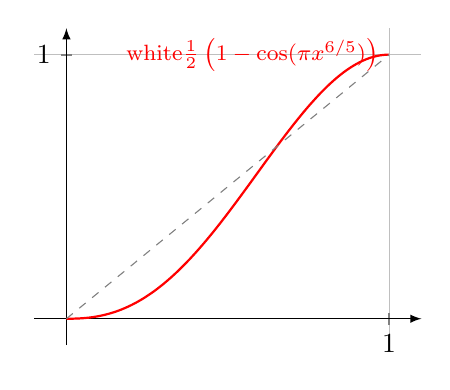
\begin{tikzpicture}
    \begin{axis}[width=6.5cm,
        axis lines=middle,
        axis line style={-latex},
        grid=major,
        xmin=-0.1, xmax=1.1,
        ymin=-0.1, ymax=1.1,
        xtick={0,1},
        xticklabels={$0$, $1$},
        ytick={0,1},
        yticklabels={$0$, $1$},
        tick style={thick},
        ticklabel style={font=\normalsize},
    ]
    \def\a{0}
    \def\b{1}
    \addplot[red,thick,samples=100,domain=\a:\b] {1/2*(1-cos(deg(pi*x^1.2)))}
    node[left,pos=1,font=\footnotesize]{\contour{white}{$\frac{1}{2}\left(1-\cos (\pi x^{6/5}) \right)$}};
    \addplot[gray,dashed,samples=100,domain=\a:\b] {x};
    \end{axis}
\end{tikzpicture}
\caption*{\centering Exemple d'une fonction vérifiant les hypothèses de l'énoncé}
\end{marginfigure}



\section{Convexité et signe}
\begin{itemize}
    \item Que peut-on dire sur une fonction concave et positive sur $\R$ ?
    \item Faire un dessin...
\end{itemize}

\section{\textsc{Rolle} à l'infini}
\begin{theo}{}
    Soit $f: \Rp \to \R$, de classe $\mathscr{C}^2$ et telle que $f(x) \xrightarrow[x \to + \infty]{} f(0)$. Alors il existe $c \in \Rpe$ et $d \in \Rp$ tel que $f'(c) = f''(d) = 0$.
\end{theo}

\section{Théorème de \textsc{Darboux}}
\begin{theo}{}
    Soit $f$ une fonction réelle, dérivable sur un intervalle $[a, b]$. Pour tout réel $k$ compris entre $f'(a)$ et $f'(b)$, il existe un réel $c \in [a, b]$ tel que $c = f'(k)$.
\end{theo}

\underline{Fonction de \textsc{Darboux}:} \\
Fonction dérivable en tout point, mais dont la dérivée est discontinue en $0$:

\begin{alignat*}{2}
    \text{Soit } f\ :\ \R\ &\longrightarrow\ \R\\
    x\ &\longmapsto\ 
    \begin{cases}
        x^2 \sin \left( \frac{1}{x^2} \right) &\text{ si } x \not= 0,\\
        0 &\text{ sinon}.
    \end{cases}
\end{alignat*}

\section{Uniforme continuité et intégrale convergente}
\begin{exercice}
    Soit $f : \Rp \to \R$ uniformément continue telle que $\int_0^{+\infty} f$ converge. Montrer que $f(x) \xrightarrow[x \to + \infty]{} 0$.
\end{exercice}

\begin{solution}
    Soit $x \in \Rp$.
    \begin{align*}
        f(x) &= f(x) - \frac{1}{2\eta_{\varepsilon}} \int_{x-\eta_{\varepsilon}}^{x+\eta_{\varepsilon}} f(t) \d t + \frac{1}{2\eta_{\varepsilon}} \int_{x-\eta_{\varepsilon}}^{x+\eta_{\varepsilon}} f(t) \d t \\
        &= \frac{1}{2\eta_{\varepsilon}} \int_{x-\eta_{\varepsilon}}^{x+\eta_{\varepsilon}} \big(f(x) - f(t) \big) \d t + \frac{1}{2\eta_{\varepsilon}} \int_{x-\eta_{\varepsilon}}^{x+\eta_{\varepsilon}} f(t) \d t \\
        |f(x)| &\leqslant \frac{1}{2\eta_{\varepsilon}} \int_{x-\eta_{\varepsilon}}^{x+\eta_{\varepsilon}} \underbrace{\big|f(x) - f(t)\big|}_{\leqslant \varepsilon} \d t + \left| \frac{1}{2\eta_{\varepsilon}} \int_{x-\eta_{\varepsilon}}^{x+\eta_{\varepsilon}} f(t) \d t \right| \\
        &\leqslant \varepsilon + \underbrace{\left|\frac{1}{2\eta_{\varepsilon}} \int_{x-\eta_{\varepsilon}}^{x+\eta_{\varepsilon}} f(t) \d t \right|}_{\mathclap{\longrightarrow 0 \text{ d'après le critère de \textsc{Cauchy}...}}}
    \end{align*}
\end{solution}

\marginnote[-7cm]{
    \begin{defi}{Continuité uniforme}
        Soit $f$ une fonction de $\R$ dans $\R$. La fonction $f$ est \emph{uniformément continue} si
        $$\forall \varepsilon > 0 \quad \exists \eta_{\varepsilon} > 0 \quad \forall(x, y) \in \R^2,$$
        $$\left( |x-y| \leqslant \eta_{\varepsilon} \implies |f(x) - f(y)| \leqslant \varepsilon \right).$$
    \end{defi}
}

\section{Lemme de \textsc{Croft}}
\marginnote[0cm]{Sources : \cite{exos_oraux} p. 259 \& \cite{oraux_x_ens_3} p. 322}

\begin{lemme}
    Soit $f : \Rp \to \R$ telle que, pour tout $a > 0$, la suite $\big(f(na) \big)_{n \geqslant 0}$ tend vers 0. \\
    Montrer que si la fonction $f$ est uniformément continue, on a $\lim\limits_{x \to + \infty} f(x) = 0$.
\end{lemme}

Sources : correction principalement de \cite{oraux_x_ens_3} avec des précisions venant de \cite{exos_oraux}.

\begin{preuve}
    L'hypothèse signifie que $f$ tend vers $0$ selon toute suite arithmétique de la forme $(na)_{n \geqslant 0}$. Lorsque la fonction est uniformément continue, on peut contrôler son comportement entre deux termes consécutifs de la suite. Plus précisément, soit $\varepsilon > 0$. La continuité uniforme de $f$ permet de choisir $\eta_\varepsilon > 0$ tel que pour tout $(x, y) \in (\Rp)^2$, 
    $$|x-y| \leqslant \eta_\varepsilon \Rightarrow |f(x) - f(y)| \leqslant \varepsilon.$$
    Puisque $\eta_\varepsilon > 0$, la suite $\big(f(n\eta_\varepsilon)\big)_{n \geqslant 0}$ tend vers $0$ par hypothèse. Fixons $N$ tel que $|f(n \eta_\varepsilon)| \leqslant \varepsilon$ pour $n \geqslant N$. \\
    Soient $x \geqslant N \eta_\varepsilon$ et $n \defeq \min\ens[\big]{ k \in \N \tq x \leqslant k \eta_\varepsilon }$ qui est bien défini. Alors $|x-n\eta_\varepsilon| \leqslant \eta_\varepsilon$. On a alors $|f(x) - f(n \eta_\varepsilon)| \leqslant \varepsilon$ de sorte que par l'inégalité triangulaire, 
    \begin{align*}
        |f(x)| &\leqslant |f(x) - f(n \eta_\varepsilon)| + |f(n \eta_\varepsilon)| \\
        &\leqslant 2 \varepsilon.
    \end{align*}
    Ceci étant valable pour tout $x \geqslant N \eta_\varepsilon$, on a bien prouvé que $f$ tend vers $0$ en $+ \infty$.
\end{preuve}  

\begin{marginfigure}[-3cm]
    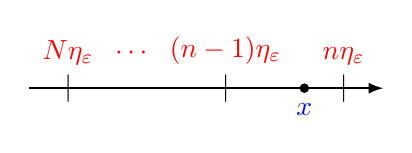
\begin{tikzpicture}[scale=5]
    \draw[-latex] [thick](-0.1,0) -- (0.8,0);
    
    \draw (0,0) node [above=5pt, red,fill=white]{$N \eta_\varepsilon$};
    \draw (0,0) node {$|$};
    
    \draw (0.16,0) node [above=7pt, red,fill=white]{$\cdots$};

    \draw (0.4,0) node [above=5pt, red,fill=white]{$(n-1) \eta_\varepsilon$};
    \draw (0.4,0) node {$|$};
    
    \draw [fill] (0.6,0) circle [radius=0.3pt];
    \draw (0.6,0) node [below=2pt, blue,fill=white]{$x$};

    \draw (0.7,0) node [above=5pt, red,fill=white]{$n \eta_\varepsilon$};
    \draw (0.7,0) node {$|$};
\end{tikzpicture}
\end{marginfigure}


\begin{exercice}
    \cite{exos_oraux} (p.261)
    Déterminer les fonctions $f \in \mathscr{C}^1(\R, \R)$ telles que $f \circ f = f$.
\end{exercice}

\begin{itemize}
    \item Equation fonctionnelle
\end{itemize}